\chapter{Numerical investigation}

\section{Perfomance of the GPU implementation of the Conjugate Gradient algorithm}

\section{Test with background mesons}

The Dirac operator for Wilson fermions in the yukawa model is
\begin{equation*}
D_{n m}=\sum_\alpha\left[\frac{\gamma_\alpha \delta_{n+\alpha, m} - \gamma_\alpha \delta_{n-\alpha, m}}{2} + (m_q + g \phi) \, \delta_{n m}\right] .
\end{equation*}
In momentum space it reads
\begin{equation*}
\bar{D}_{f f^{\prime}}(p)=\left(m+ g \sigma \sum_\mu 2 \sin ^2\left(\frac{p_\mu}{2}\right)+i \sum_\mu \gamma_\mu \sin \left(p_\mu\right)\right) \delta_{f f^{\prime}}
\end{equation*}
The inverse can be checked to be 
\begin{equation*}
    \bar D_{f,f'} ^{-1} = \left[m + \dots\right] \ \left(m+ g \sigma \sum_\mu 2 \sin ^2\left(\frac{p_\mu}{2}\right) - i \sum_\mu \gamma_\mu \sin \left(p_\mu\right)\right) \delta_{f f^{\prime}}
\end{equation*}
One can now find the pole mass by imposing $D^{-1} = 0$ and gets 
\begin{equation*}
    m + \dots = 0
\end{equation*}

\section{Classical to quantum interpolation}
\label{sec:classical_to_quantum}

Let us start by analising the coloured noise field in the simulation and relevant properties that emerge from it. We consider the Yukawa model described by the continuum action \ref{eq:yukaw_continuum}.
In figure \ref{fig:thermalisation_different_noise_fracs} the system is initialised in the same state for all the configurations, and then evolved with the Langevin equation with various noise fractions. The red line corresponds to the case $s=0$, namely a classical simulation. The blue line corresponds to the case $s=1$, namely the fully quantum case. As one can notice, the introduction of noise shifts the equilibrium expectation value of the field monotonically with the cutoff fraction: this is due to the fact that WHAT???. Note that a lower noise fraction is correlated to a faster convergence towards equilibrium. Moreover, low-distance fluctuations are suppressed due to the removal of the ultraviolet modes in the noise term.
\begin{figure}
    \centering
    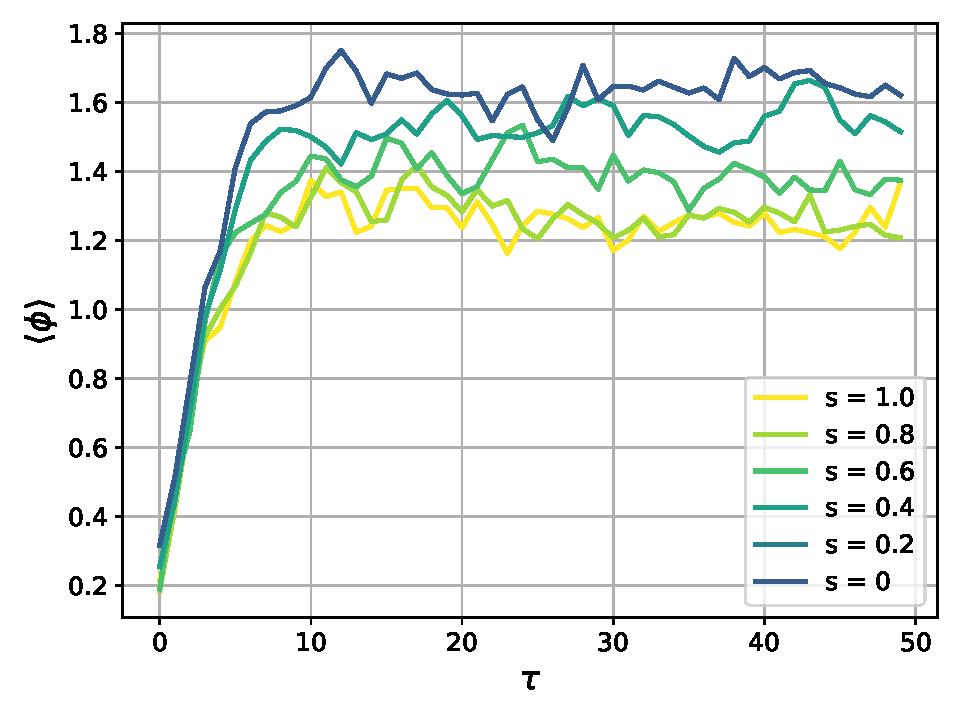
\includegraphics[scale=0.7]{figures/thermalisation.pdf}
    \caption{Thermalisation for different noise fractions}
    \label{fig:thermalisation_different_noise_fracs}
\end{figure}

For $\lambda = 0$ one has
\begin{equation}
    \sigma = -\frac{g}{m_\phi^2 + k^2} \, \bar\psi \psi
    \label{eq:equation_motion_NJL_no_self_interaction}
\end{equation}
In figure \ref{fig:equation_motion_NJL} one can see that equation \eqref{eq:equation_motion_NJL_no_self_interaction} is verified also on the fully quantum level.
\begin{figure}
    \centering
    \includegraphics{}
    \caption{Caption}
    \label{fig:equation_motion_NJL}
\end{figure}


Figures \ref{fig:slide_broken_phi} - \ref{fig:slide_broken_mphir} report a few observables as a function of the cutoff fraction $s$. In this case all the coupling constants are kept fixed while changing the value of $s$, in order to provide a smooth interpolation between the fully classical and fully quantum picture. \\
Each figure reports two plots corresponding to two different parameter configurations. The COLOR1 line corresponds to a system in the symmetric phase, while the COLOR2 line correspond to the broken phase. The exact parameters for the two configurations are reported under the figure.
\begin{figure}
    \centering
    \begin{minipage}{0.45\textwidth}
        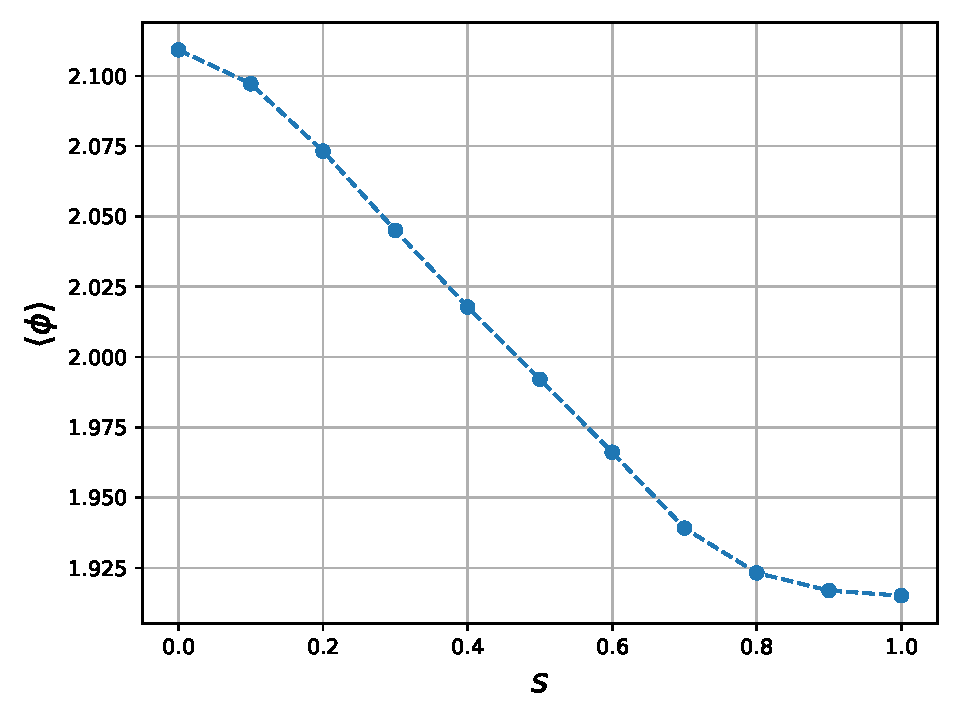
\includegraphics[scale=0.52]{figures/slide_broken/phi.pdf}
        \captionof{figure}{phi}
        \label{fig:slide_broken_phi}
    \end{minipage}
    \hfill
    \begin{minipage}{0.45\textwidth}
        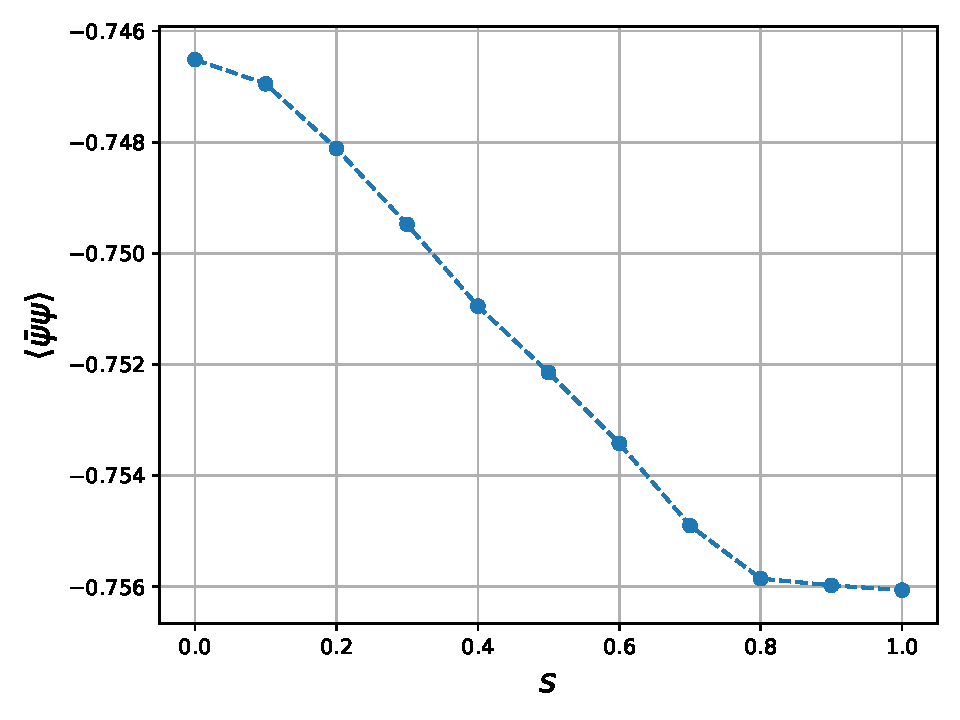
\includegraphics[scale=0.52]{figures/slide_broken/cond.pdf}
        \captionof{figure}{cond}
        \label{fig:slide_broken_cond}
    \end{minipage}
 \begin{minipage}{0.45\textwidth}
    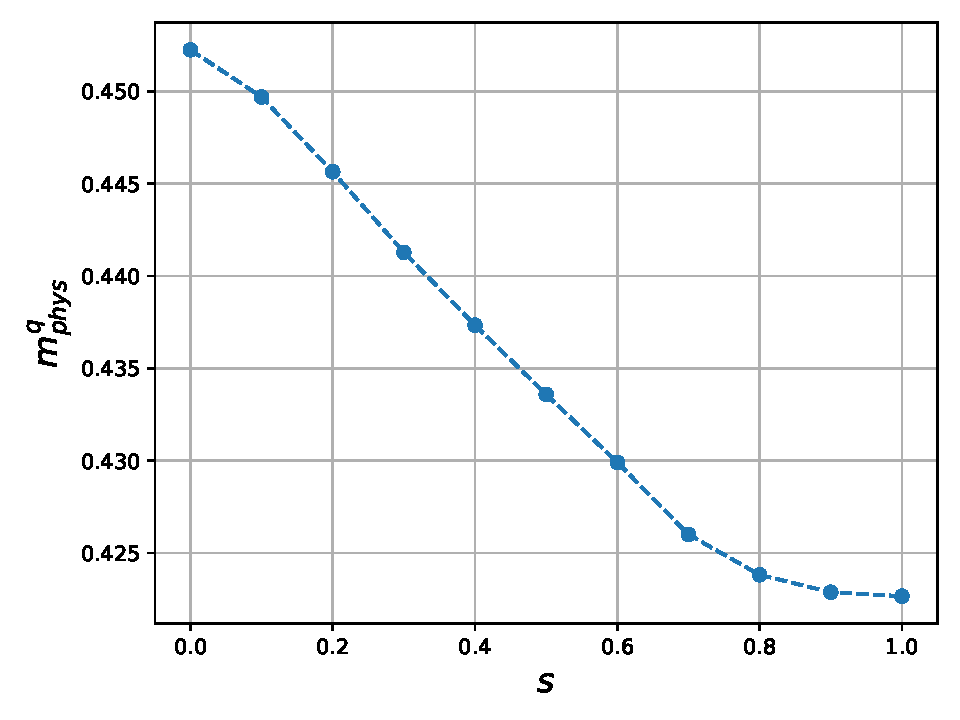
\includegraphics[scale=0.52]{figures/slide_broken/mqphys.pdf}
    \captionof{figure}{mqphys}
    \label{fig:slide_broken_mqphys}
\end{minipage}
\hfill
\begin{minipage}{0.45\textwidth}
    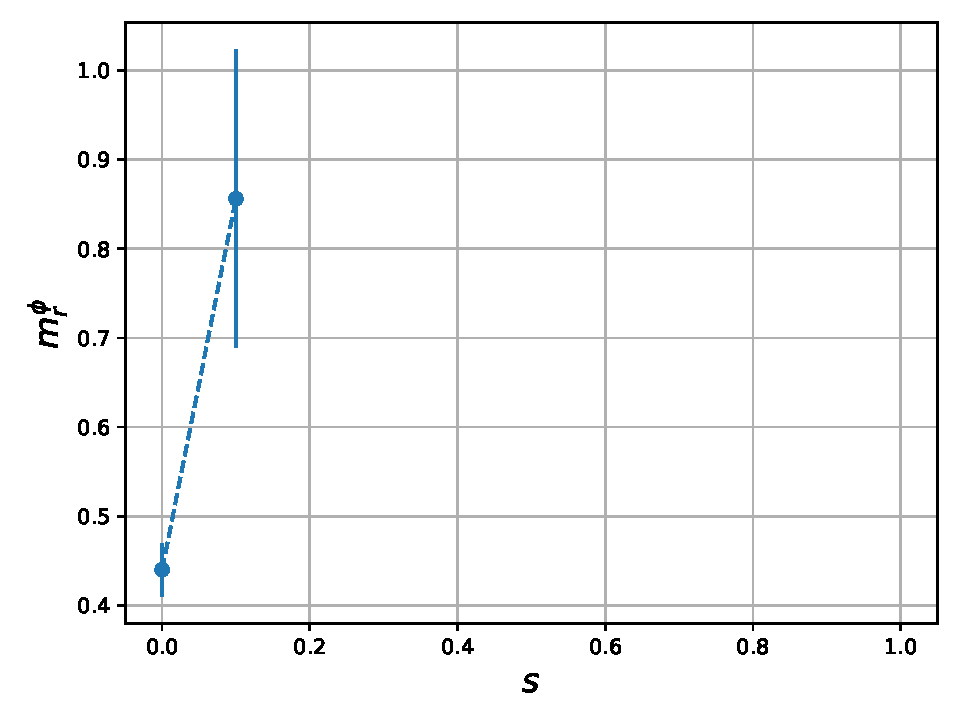
\includegraphics[scale=0.52]{figures/slide_broken/mphir.pdf}
    \captionof{figure}{mphir}
    \label{fig:slide_broken_mphir}
\end{minipage}
\caption{slide broken}
\label{fig:slide_broken}
\end{figure}

\section{Chiral fermions and the chiral phase transition}

\section{Cooling with coloured noise}
In this section we report and discuss results of the NJL model and Quark-Meson model using the technique of coloured noise to perform block-spin steps as outlined in the paragraph \ref{sec:coloured_noise}. We first set up the white noise simulation with $s=1$ on a lattice of size $8 \times 8$, with spacing $a$ and cutoff $\Lambda$. We then start performing complete block-spin steps as summarised in table \ref{tab:block_spin_steps}. \\

Figure \ref{fig:yukawa_scan_phi}, \ref{fig:yukawa_scan_chi2} report the analysis of the system for various values of the Yukawa coupling $g$. The classical equation of motion \eqref{eq:eq_motion_NJL} is invariant under the transformation $g \to -g, \sigma \to -\sigma$. This means that one should expect, from a classical point of view, the order parameter $\sigma$ to be anti-symmetric around $g = 0$. By looking at figrue \ref{fig:yukawa_scan_phi}, one can conclude that the symmetry is still present on the quantum level, but around a point $g_0 \neq 0$ which is solution of the equation $\left\langle \sigma \right\rangle = 0$. DOES THE POINT $g_0$ IDENTIFY A PHASE TRANSITION?

\begin{figure}[h]
    \centering
    \begin{minipage}{0.45\textwidth}
        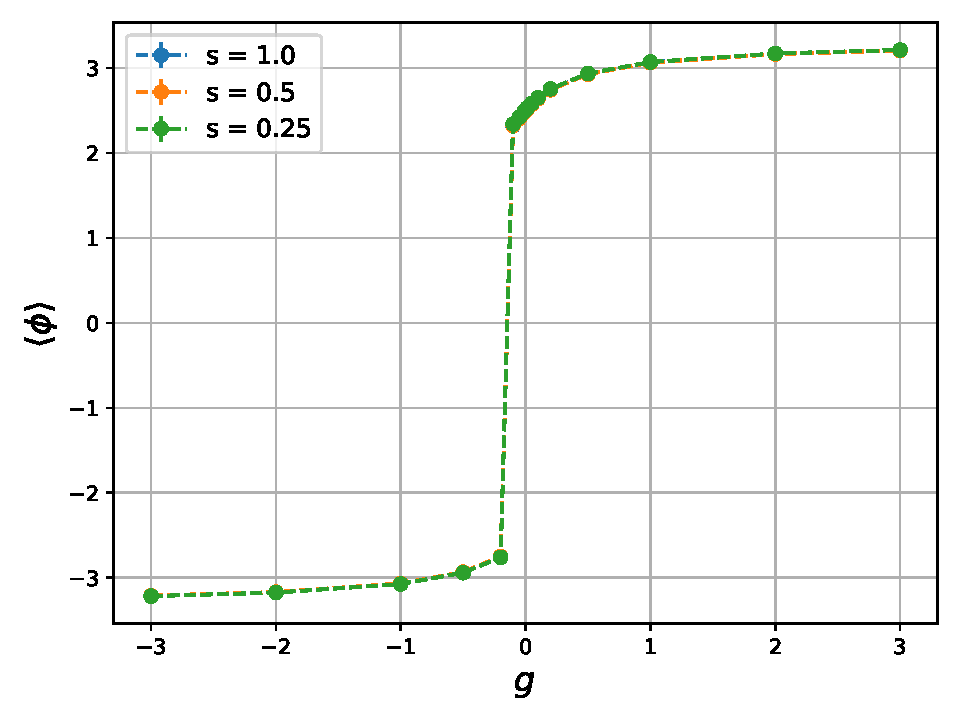
\includegraphics[scale=0.5]{figures/yukawa_scan/phi.pdf}
        \captionof{figure}{Magnetisation}\label{fig:yukawa_scan_phi}
    \end{minipage}
    \hfill
    \begin{minipage}{0.45\textwidth}
        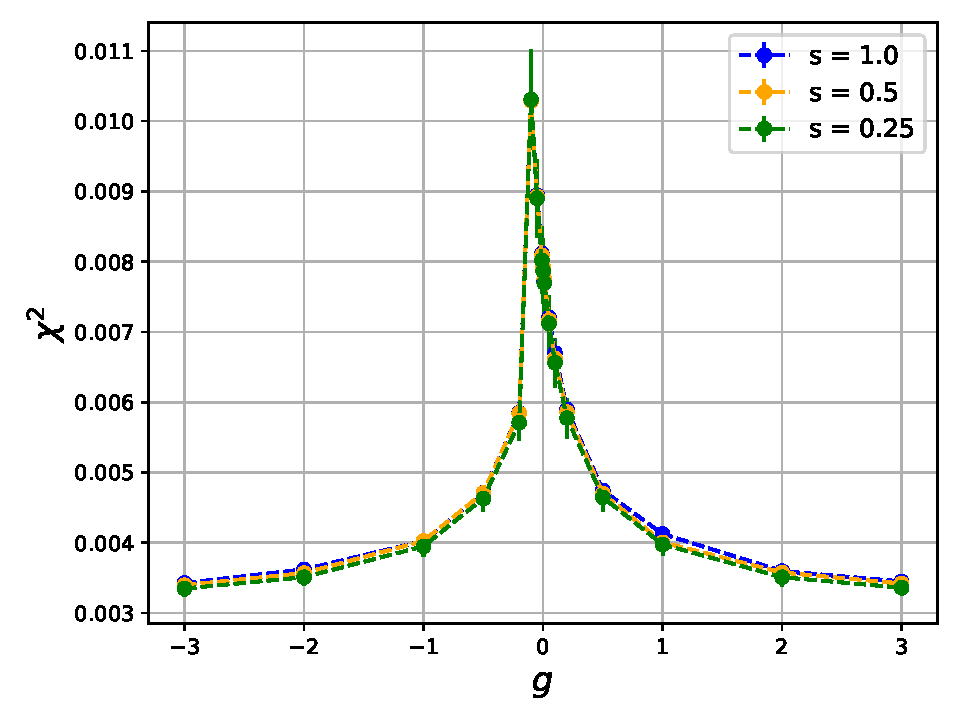
\includegraphics[scale=0.5]{figures/yukawa_scan/chi2.pdf}
        \captionof{figure}{Susceptibility}\label{fig:yukawa_scan_chi2}
    \end{minipage}
\end{figure}

As one can see, for the first two block spins there is perfect agreement among the various curves. From the third step, some small deviation comes in due to the momentum dependence of the coupling.


\begin{figure}
    \centering
    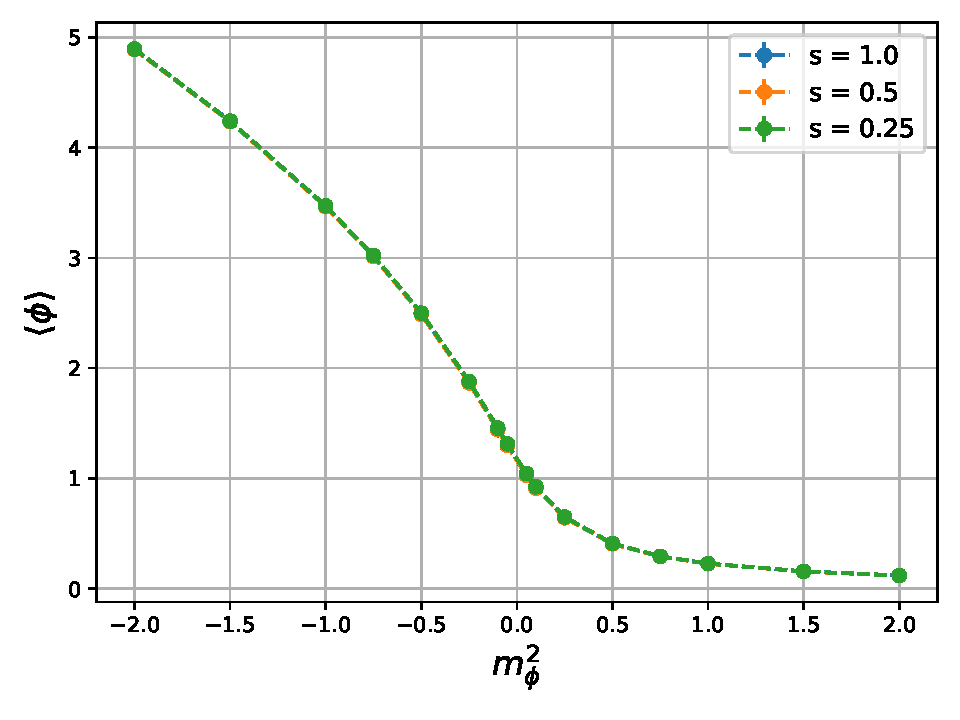
\includegraphics[scale=0.7]{figures/phase_trans/phi.pdf}
    \caption{}
    \label{fig:bs_NJL_magnetisation_yukawa}
\end{figure}

Perhaps more interesting are the plots in figure \ref{fig:bs_NJL_quantities_mass}, reported as a function of the bare mesons mass. 
The peek in the magnetic susceptibility deserves some comment. In general, in a finite-volume lattice theory, no phase transition can happen. To state the presence of a phase transition, one should look at the infinite volume limit, which is done by studying the volume scaling of the magnetic susceptibility. In particular we do not expect a phase transition in our model due to the spontaneous breaking of the $O(1)$ symmetry, since the presence of a finite bare quark mass already breaks the $O(1)$ symmetry explicitly. As a remark to this statement, we studied the volume scaling of $\chi$, as reported in figure \ref{fig:chi_volume_scaling}. It is clear that it converges towards XXX, implying that the system is not undergoing a phase transition.

\begin{figure}
    \centering
    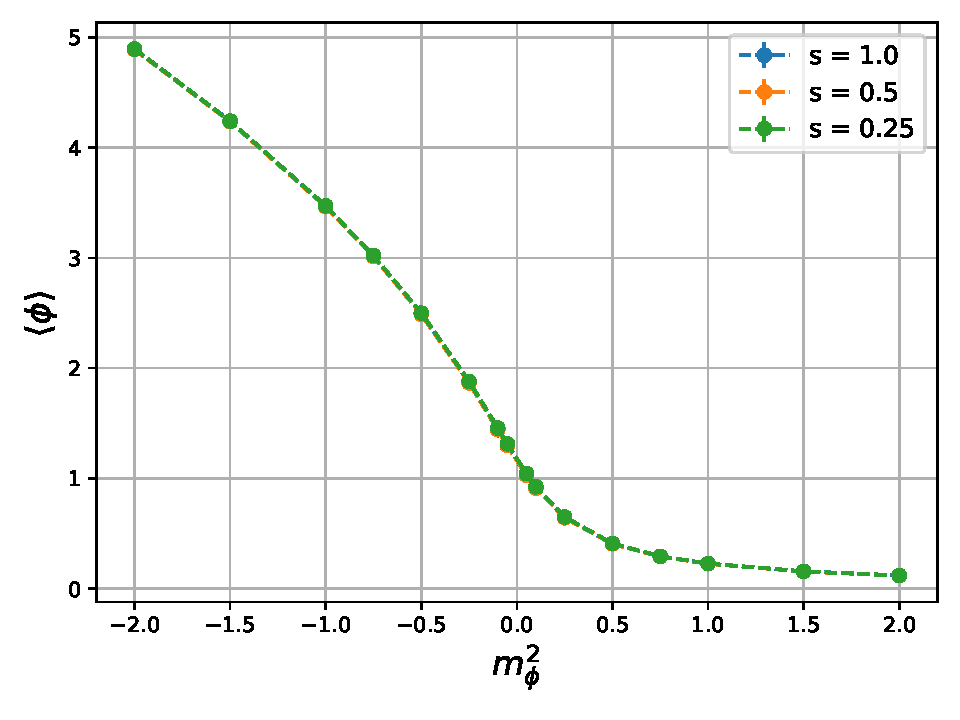
\includegraphics[scale=0.7]{figures/phase_trans/phi.pdf}
    \caption{}
    \label{fig:bs_NJL_quantities_mass}
\end{figure}

\begin{figure}
    \centering
    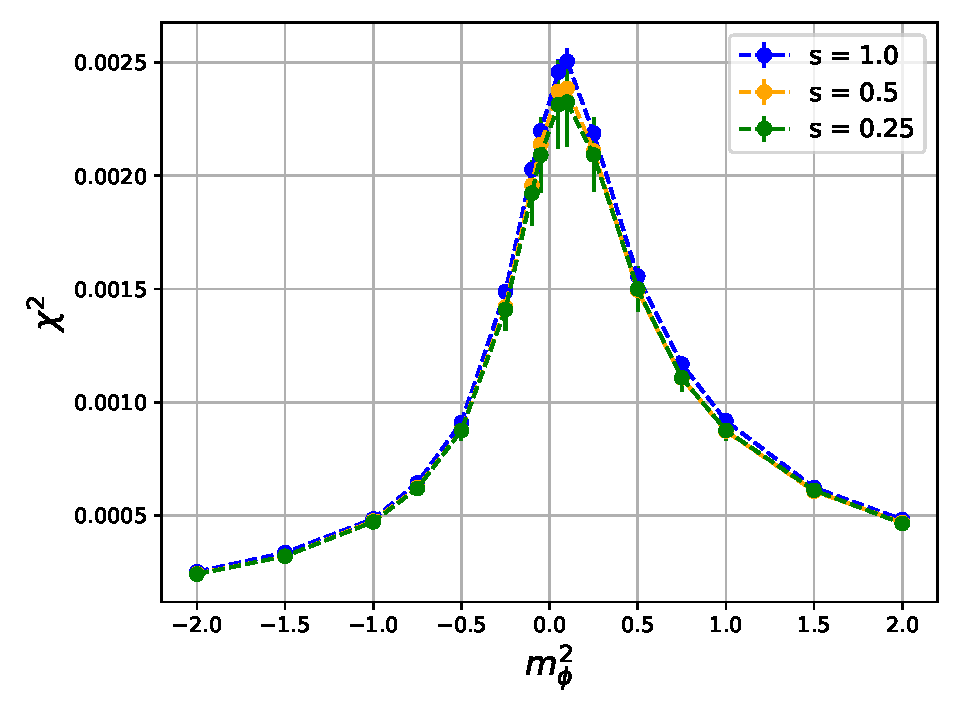
\includegraphics[scale=0.7]{figures/phase_trans/chi2.pdf}
    \caption{}
    \label{fig:chi_volume_scaling}
\end{figure}


Look at various things such as magnetization, mass, etc. \\
Even though is O(1) we do not observe SSB because of fermion bare quark mass. \\
Peak in the susceptibility does not imply P.T. $\rightarrow$ look at volume scaling. \\
When does L.O. rescaling ansatz breaks down?


\newpage

\begin{equation*}
    S[\phi, \bar\psi, \psi] = \int_x \phi \left(\frac{\partial^2}{2} + \frac{m_\phi^2}{2}\right) \phi + \frac{\lambda}{4!} \phi^4 + \bar \psi \left(\slashed{\partial} + m_q + g\phi\right) \psi
\end{equation*}

\begin{equation*} 
    \lambda = 1.0 \qquad m_\Phi^2 = 0.5 \qquad N_t \times N_x = 8 \times 32 \qquad m_q = 0.5 \qquad N_{conf} = 5 \cdot 10^3 \qquad \bar\epsilon = 0.01
\end{equation*}

\begin{figure}[h]
    \centering
    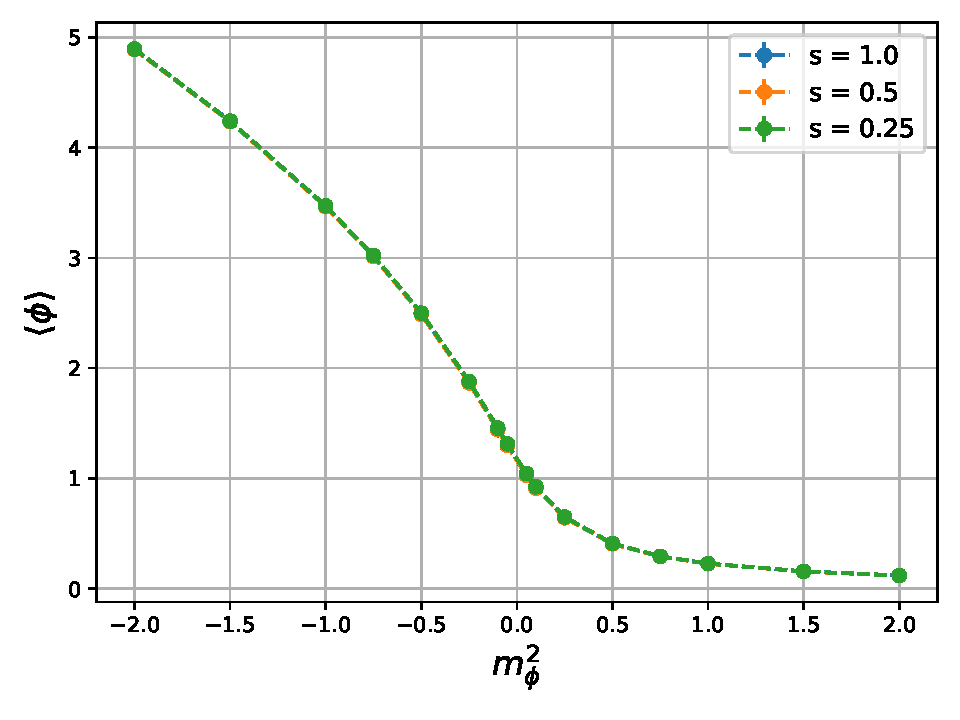
\includegraphics[scale=0.7]{figures/phase_trans/phi.pdf}
    \caption{Magnetization}
    \label{fig:enter-label}
\end{figure}

\begin{figure}[h]
    \centering
    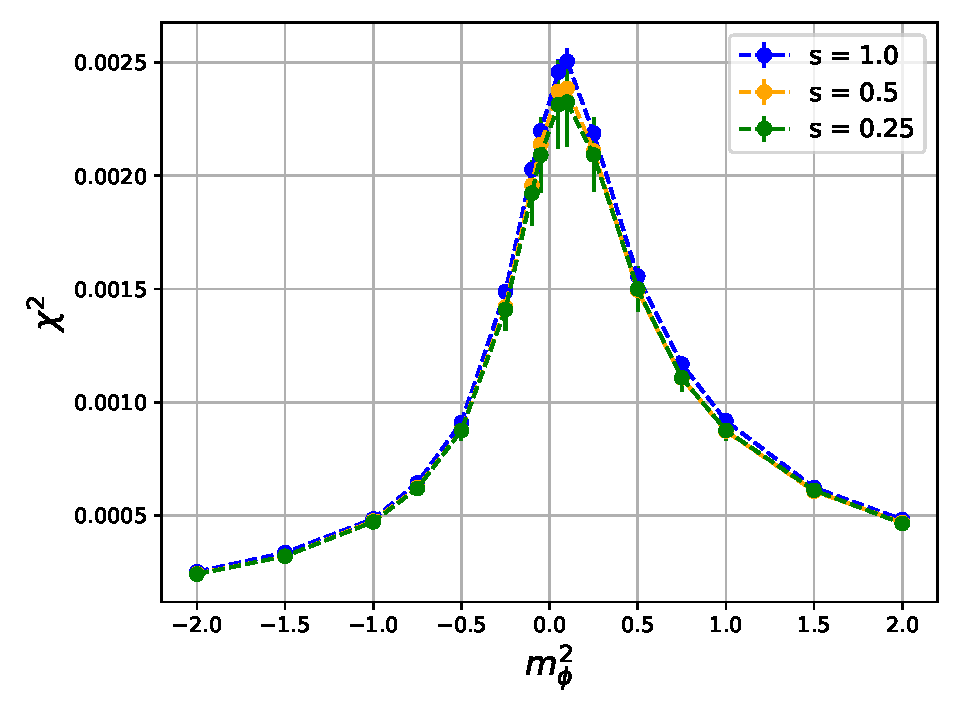
\includegraphics[scale=0.7]{figures/phase_trans/chi2.pdf}
    \caption{Magnetic susceptibility}
    \label{fig:enter-label}
\end{figure}

\begin{figure}[h]
    \centering
    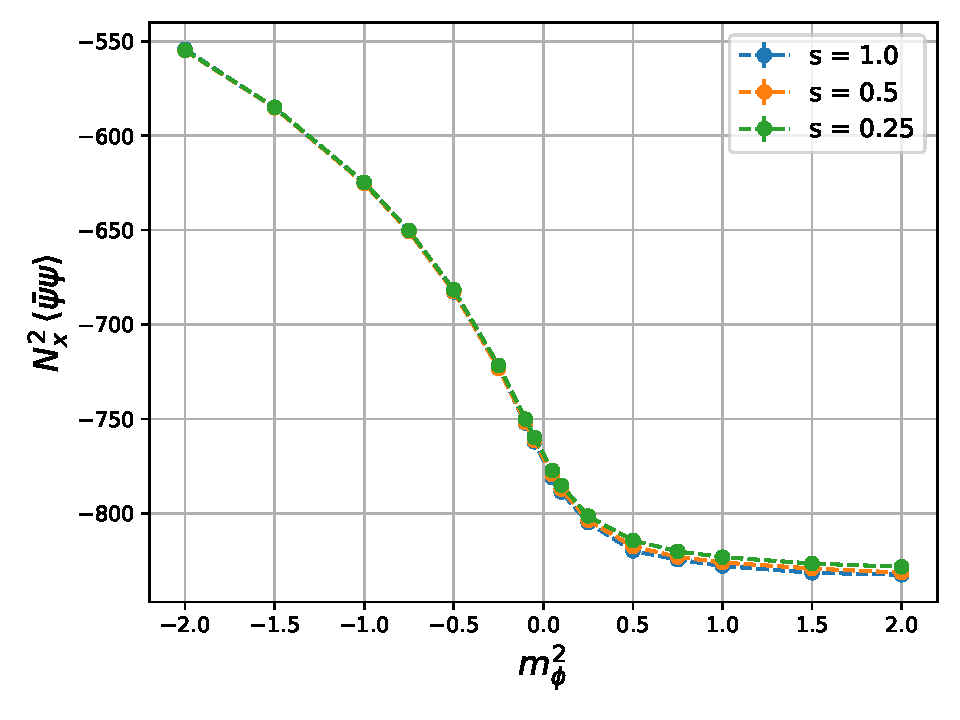
\includegraphics[scale=0.7]{figures/phase_trans/condensate.pdf}
    \caption{Condensate}
    \label{fig:enter-label}
\end{figure}